\begin{cuzchapter}{系统需求分析}{chap:requirement}
\section{需求概述}
APPT 是一个 AI 驱动的幻灯片协作编辑平台，旨在为用户提供便捷的在线幻灯片创作、实时协作、AI 内容生成和版本管理等功能。系统需支持多用户同时编辑同一份幻灯片文档，提供语法高亮、实时预览、评论讨论以及基于角色的权限控制。此外，管理员负责用户注册码的生成、用户状态管理以及系统主题与插件的维护。整个系统需具备高可用性、数据安全性和良好的用户体验。

\section{系统功能性需求}
系统功能分为用户端和管理员端。
注册用户可创建和管理幻灯片空间与文档，
利用 Markdown 进行内容编写并实时预览；
支持多人实时协作编辑、评论、版本回溯以及 AI 辅助生成内容。
管理员除继承全部用户功能外，还负责用户与注册码管理、主题与插件维护。
如图\ref{fig:user-case-diagram-for-user}
    \begin{figure}[htbp]
        \centering
        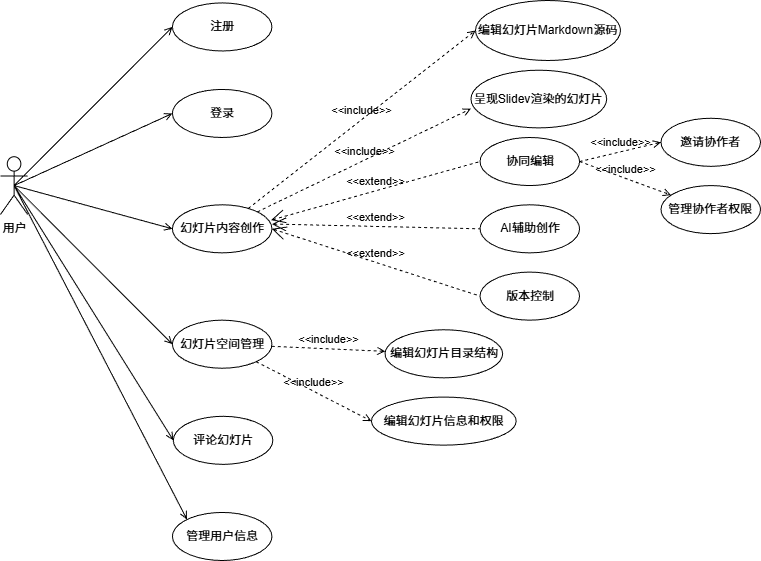
\includegraphics[width=0.9\textwidth]{figures/drawio/用户用例图.drawio.png}
        \caption{用户模块功能需求用例图}
        \label{fig:user-case-diagram-for-user}
    \end{figure}
\begin{figure}


\end{figure}
\section{系统非功能性需求}
\begin{itemize}
    \item \textbf{性能要求}：在 50 人同时在线协作编辑时，编辑操作的同步延迟应低于 200 ms；Markdown 预览渲染时间不超过 500 ms。
    \item \textbf{可用性}：系统应提供 99.9\% 的服务可用性，支持 7×24 小时不间断运行。
    \item \textbf{安全性}：所有 API 请求需通过 JWT 身份认证，密码使用 bcrypt 哈希存储；文档访问须严格遵循 Owner/Editor/Commenter/Viewer 四级权限控制；WebSocket 连接在握手阶段完成令牌验证。
    \item \textbf{可扩展性}：后端微服务模块应支持水平扩展，数据库连接池需根据负载动态调整；前端组件应采用可复用设计，便于后续功能迭代。
    \item \textbf{可维护性}：代码需遵循 TypeScript 严格模式，后端提供 Swagger API 文档，前端关键逻辑应包含单元测试。
    \item \textbf{兼容性}：支持 Chrome、Firefox、Safari 及 Edge 最新两个主要版本；移动端浏览器需提供基本的查看与评论功能。
\end{itemize}
\end{cuzchapter}